\documentclass{article}

\usepackage{mathtools, amsthm, amssymb, amsmath}

\usepackage[sloppy=false, thaifont=TH Sarabun New]{thaispec}
\usepackage[a4paper,margin=1in]{geometry}

\usepackage[style=numeric, sorting=none]{biblatex}
\addbibresource{math_model.bib}

\usepackage{graphicx}
\graphicspath{{./picture/}}

\usepackage{multirow}

\title{แบบจำลองทางคณิตศาสตร์การเรียนรู้ตัวอักษรคันจิ}
\author{
\begin{tabular}{ll}
    นายณัฐวุฒิ เทศงามถ้วน & 116410901009-3 \\
    นายคณัสนันท์ ทรัพย์อุดม & 116410901033-3 \\
    นายธนาคาร ธิคุณ & 116410901048-1
\end{tabular}
}
\date{2 กุมภาพันธ์ 2565}

\begin{document}

\maketitle
\tableofcontents
\listoffigures

\begin{abstract}
แบบจำลองทางคณิตศาสตร์การเรียนรู้ตัวอักษรคันจิ เป็นแบบจำลองที่ถูกออกแบบมาเพื่อให้สามารถวิเคราะห์ผลการเรียนรู้คันจิ เวลาที่ใช้ในการเรียนรู้ตัวอักษรคันจิ และตอบโจทย์ปัญหาภายในหลักสูตรการศึกษาได้ว่าต้องเรียนรู้คันจิเท่าใดต่อวันจึงจะสามารถเรียนรู้คันจิได้ครบทุกตัวอักษร เพื่อให้ได้ซึ่งหลักสูตรการเรียนรู้ตัวอักษรคันจิที่มีประสิทธิมากยิ่งขึ้น
\end{abstract}

\section{บทนำ}
ปัจจุบันประเทศไทยได้รับอิทธิพลทางสังคมและวัฒนธรรมมาจากต่างประเทศ โดยเฉพาะจากญี่ปุ่นเป็นอย่างมาก จึงจำเป็นต้องผลิตบุคลากรที่มีความเข้าใจสังคมและวัฒนธรรมของประเทศญี่ปุ่นอันจะนำไปสู่การสามารถติดต่อสื่อกับชาวญี่ปุ่นได้อย่างราบรื่นและสร้างความสัมพันธ์อันดีต่อกัน\cite{หลักสูตรสาขาวิชาภาษาญี่ปุ่น2561}

จากที่กล่าวข้างต้น ทำให้เราเล็งเห็นถึงปัญหาหนึ่งที่สำคัญเป็นอย่างยิ่งในการเรียนรู้วัฒนธรรมของประเทศญี่ปุ่นนั้นก็คือ การที่ประเทศญี่ปุ่นใช้ตัวอักษรคันจิในการสื่อสารในชีวิตประจำวัน โดยคันจิหมายถึงตัวอักษรภาพที่ประเทศจีนและประเทศญี่ปุ่นมีใช้ร่วมกันเพื่อใช้ในการสื่อสารกันในสังคมของประเทศตนเอง ดังนั้นการที่เราจะเข้าใจถึงสังคมและวัฒนธรรมได้นั้นไม่เพียงแต่จะต้องเข้าใจไวยากรณ์ แต่ต้องเข้าใจถึงตัวอักษรคันจิที่สามารถสื่อได้ถึงความหมายด้วยจึงจะสามารถบรรลุผลการศึกษาภาษาญี่ปุ่นเพื่อติดต่อสื่อกับชาวญี่ปุ่นได้อย่างราบรื่นและสร้างความสัมพันธ์อันดีต่อกัน

เมื่อเราทราบถึงปัญหาแล้ว โจทย์ที่เราจะต้องแก้ปัญหาให้ได้นั้นก็คือ จะสร้างแบบจำลองทางคณิตศาสตร์อย่างไรเพื่อให้สามารถพยากรณ์วันเวลาทั้งหมดที่ใช้ในการเรียนรู้ตัวอักษรคันจิและสามารถหาจำนวนตัวอักษรคันจิที่ควรเรียนภายใต้เวลาเรียนที่กำหนด ซึ่งถือว่าเป็นประเด็นสำคัญในการทำแบบจำลองทางคณิตศาสตร์ในหัวข้อการเรียนรู้ตัวอักษรคันจิ

ดังนั้นกลุ่มเราจึงได้จัดทำแบบจำลองทางคณิตศาสตร์การเรียนรู้ตัวอักษรคันจิ เพื่อให้สามารถศึกษาการเรียนรู้ตัวอักษรคันจิที่เหมาะสมได้รวมถึงหาจำนวนตัวอักษรคันจิที่ควรเรียนภายใต้เวลาเรียนที่กำหนด ซึ่งจะช่วยให้หลักสูตรสาขาวิชาภาษาญี่ปุ่นสามารถปรับหลักสูตรได้ตรงกับปัญหาได้มากยิ่งขึ้น โดยแบบจำลองทางคณิตศาสตร์การเรียนรู้ตัวอักษรคันจิของเราจะนำเอาหลักสูตรสาขาวิชาภาษาญี่ปุ่นของมหาวิทยาลัยมหาวิทยาลัยธรรมศาสตร์มาเป็นโจทย์ในการทำแบบจำลองทางคณิตศาสตร์

\section{ความรู้พื้นฐานที่จำเป็น}
ในการจะสร้างแบบจำลองทางคณิตศาสตร์การเรียนรู้ตัวอักษรคันจิได้นั้น จำเป็นจะต้องอาศัยข้อมูลวิชาที่เรียนรู้ตัวอักษรคันจิจากหลักสูตรสาขาวิชาภาษาญี่ปุ่นโดยได้มาจากมหาวิทยาลัยธรรมศาสตร์ซึ่งมีข้อมูลดังต่อไปนี้ 
\break
รายวิชาเรียนที่เกี่ยวข้องกับตัวอักษรคันจิของมหาวิทยาลัยธรรมศาสตร์ โดยแบ่งออกเป็น 6 ภาคเรียน ภาคเรียนละวิชาดังนี้
\begin{enumerate}
	\item วิชา Japanese 1 : มีกำหนดการเรียนรู้ตัวอักษรคันจิทั้งหมด 80 ตัว ไม่มีเงื่อนไขวิชาที่ต้องเรียนก่อน Japanese 1
	\item วิชา Japanese 2 : มีกำหนดการเรียนรู้ตัวอักษรคันจิทั้งหมด 120 ตัว มีเงื่อนไขวิชาที่ต้องเรียนก่อน Japanese 2 คือ ต้องเรียนวิชา Japanese 1 ผ่านมาก่อนวิชานี้
	\item วิชา Japanese 3 : มีกำหนดการเรียนรู้ตัวอักษรคันจิทั้งหมด 250 ตัว มีเงื่อนไขวิชาที่ต้องเรียนก่อน Japanese 3 คือ ต้องเรียนวิชา Japanese 2 ผ่านมาก่อนวิชานี้
	\item วิชา Japanese 4 : มีกำหนดการเรียนรู้ตัวอักษรคันจิทั้งหมด 250 ตัว มีเงื่อนไขวิชาที่ต้องเรียนก่อน Japanese 4 คือ ต้องเรียนวิชา Japanese 3 ผ่านมาก่อนวิชานี้
	\item วิชา Japanese 5 : มีกำหนดการเรียนรู้ตัวอักษรคันจิทั้งหมด 300 ตัว มีเงื่อนไขวิชาที่ต้องเรียนก่อน Japanese 5 คือ ต้องเรียนวิชา Japanese 4 ผ่านมาก่อนวิชานี้
	\item วิชา Japanese 6 : มีกำหนดการเรียนรู้ตัวอักษรคันจิทั้งหมด 350 ตัว มีเงื่อนไขวิชาที่ต้องเรียนก่อน Japanese 5 คือ ต้องเรียนวิชา Japanese 4 ผ่านมาก่อนวิชานี้
	\item ตัวอักษรคันจิที่ไม่ได้อยู่ในรายวิชา Japanese 1 ถึง Japanese 6 ให้ผู้เรียนศึกษาด้วยตนเองเป็นตัวอักษรคันจิอีก 786 ตัว
\end{enumerate}
โดยที่แต่ละวิชาจะเรียนตัวอักษรคันจิไม่ซ้ำกันรวมทั้งหมด 1350 ตัว และผู้เรียนสามารถศึกษาตัวอักษรคันจิได้ด้วยตนเองอีก 786 ตัว ในระหว่างภาคการศึกษาได้

นอกจากความรู้ที่เกี่ยวกับหลักสูตรสาขาวิชาภาษาญี่ปุ่น เรายังจำเป็นที่จะต้องรู้หลักการ The Forgetting Curve\cite{ebbinghaus1913memory} ซึ่งเป็นหลักการที่อธิบายการเรียนรู้ของมนุษย์ที่ถ้ามนุษย์เรียนรู้สิ่งใดสิ่งหนึ่งไปแล้วจะค่อยๆ หลงลืมตามเวลาที่ผ่านไป โดยจากการทดสอบพบว่า หากมนุษย์เราเรียนรู้สิ่งใดสิ่งหนึ่งมาแล้วแต่ไม่ได้กลับไปทบทวนซ้ำเป็นเวลา 1 วัน สิ่งที่มนุษย์คนนั้นได้เรียนรู้มาจะเหลืออยู่ 33.7\% เท่านั้น ซึ่งสามารถนำมาใช้ประยุกต์กับการทำแบบจำลองทางคณิตศาสตร์การเรียนรู้ตัวอักษรคันจิในส่วนของการลืมตัวอักษรคันจิที่เคยเรียนไปแล้วได้

สิ่งสุดท้ายที่จำเป็นสำหรับการทำแบบจำลองทางคณิตศาสตร์ของเรานั้นจะขาดไปไม่ได้นั้นคือ ความรู้พื้นฐานจากวิชาการสร้างตัวแบบทางคณิตศาสตร์\cite{MathematicalModeling} ที่เป็นแหล่งอ้างอิงแบบจำลองทางคณิตศาสตร์แบบต่างๆ ที่ช่วยให้เราสามารถทำแบบจำลองทางคณิตศาสตร์การเรียนรู้ตัวอักษรคันจิให้ดีได้มากยิ่งขึ้น

\section{ผลลัพธ์หลัก}
จากข้อมูลที่มีในความรู้พื้นฐานที่จำเป็นทำให้เราสามารถทำแบบจำลองทางคณิตศาสตร์การเรียนรู้ตัวอักษรคันจิได้ดังนี้

\subsection{ปัญหา} 
การหาสมการที่ใช้ทำนายผลการเรียนรู้ตัวอักษรคันจิและถ้าต้องเรียนรู้ตัวอักษรคันจิภายในระยะเวลา 720 วัน จะต้องเรียนรู้ตัวอักษรคันจิกี่ตัวต่อวันถึงจะเรียนรู้ตัวอักษรคันจิครบทั้งหมด 2136 ตัว
\begin{figure}[b]
\centering
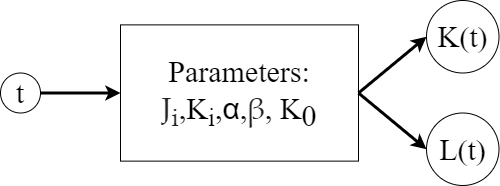
\includegraphics[scale=0.5]{1.png}
\caption{ภาพแสดงตัวแปรในโจทย์}
\label{fig:inoutput}
\end{figure}
\subsection{องค์ประกอบ}
\begin{center}
\begin{tabular}{ |c|c|c|c| }
\hline
\textbf{สัญลักษณ์ } & \textbf{ประเภท } & \textbf{ตัวแปร } & \textbf{หน่วย } \\
\hline
$L(t)$ & ตัวแปรผลลัพธ์ & ตัวอักษรคันจิที่ผู้ศึกษารู้ ณ วันที่ t & ตัว \\
\hline
$L_i(t)$ & พารามิเตอร์ & ตัวอักษรคันจิที่ผู้ศึกษารู้ในช่วงเวลาเรียน Japanese i ณ วันที่ t & ตัว \\
\hline
$K_i$ & พารามิเตอร์ & ตัวอักษรคันจิที่สามารถเรียนรู้ได้ด้วยตนเอง ณ เวลาเรียน Japanese i & ตัว \\
\hline
$t$ & ตัวแปรนำเข้า & เวลาในการเรียนรู้ตัวอักษรคันจิ & วัน \\
\hline 
$J_i$ & พารามิเตอร์ & ตัวอักษรคันจิทั้งหมดที่สามารถเรียนรู้ได้ในช่วงเวลาเรียน Japanese i & ตัว \\
\hline
$K_{0,i}$ & พารามิเตอร์ & ตัวอักษรคันจิที่ผู้ศึกษามีความรู้และจำได้อยู่แล้วในวิชา Japanese i & ตัว \\
\hline
$\alpha$ & พารามิเตอร์ & ความสามารถในการเรียนรู้ตัวอักษรคันจิต่อวัน & ตัว/วัน \\
\hline 
$\beta $ & พารามิเตอร์ & อัตราการสูญเสียตัวอักษรคันจิ & ไม่มี \\
\hline 
\end{tabular}
\end{center}
\subsection{สมมติฐาน}
\begin{itemize}
	\item[-] เวลาที่ใช้ในการเรียนรู้ตัวอักษรคันจิจะใช้เวลาเรียนทั้งหมด 6 ภาคเรียน ภาคเรียนละ 4 เดือน และเดือนละ 30 วัน โดยกำหนดให้การเรียน Japanese 1 อยู่ในช่วงเวลาวันที่ 1 ถึงวันที่ 120 Japanese 2 อยู่ในช่วงเวลาวันที่ 121 ถึงวันที่ 240 Japanese 3 อยู่ในช่วงเวลาวันที่ 241 ถึงวันที่ 360 Japanese 4 อยู่ในช่วงเวลาวันที่ 361 ถึงวันที่ 480 Japanese 5 อยู่ในช่วงเวลาวันที่ 481 ถึงวันที่ 600 Japanese 6 อยู่ในช่วงเวลาวันที่ 601 ถึงวันที่ 720 และตัวอักษรคันจิที่ไม่ได้อยู่ในรายวิชาสามารถเรียนได้ภายในช่วงเวลา 6 ภาคเรียน
	\item[-] การเรียนรู้ตัวอักษรคันจิในแต่ละวันสามารถหลงลืมตัวอักษรคันจิที่เคยเรียนรู้ได้ด้วยหลักการ The Forgetting Curve\cite{ebbinghaus1913memory} 
	\item[-] ผู้เรียนคันจิอยู่ในสถานะที่เรียนรู้ตัวอักษรคันจิตลอดเวลา เนื่องจากสภาวะการเรียนรู้ภาษาญี่ปุ่นต้องใช้เวลาไปกับการอยู่กับตัวอักษรคันจิเป็นจำนวนมากเพื่อให้คุ้นเคยกับภาษาญี่ปุ่นตลอดเวลา
	\item[-] เวลาที่ใช้ในการเรียนรู้ตัวอักษรคันจิจะไม่นับเวลาช่วงปิดเทอมเข้ามาเกี่ยวข้อง โดยถือว่าการเรียนรู้ตัวอักษรคันจิจะเรียนรู้แบบต่อเนื่องจนกว่าจะครบทั้งหมด 6 ภาคเรียน
\end{itemize}
\subsection{แบบจำลองทางคณิตศาสตร์}
\subsubsection{แบบจำลองทางคณิตศาสตร์การเรียนรู้ตัวอักษรคันจิ}
กำหนดให้ $ K_i , K_{0,i} , t \in \mathbb{N} , \alpha , \beta \in \mathbb{R}^+ $ และ 
$$ L(t) = L_1(t) + L_2(t) + L_3(t) + L_4(t) + L_5(t) + L_6(t) $$
โดยที่
\begin{center}
\begin{align*}
L_1(t) & = \min \{J_1 + K_1, \left\lfloor (1 - \beta)(K_{0,1} + \alpha{t}) \right\rfloor\} \; ; t \in (0,120] \\
L_2(t) & = \min \{J_2 + K_2, \left\lfloor (1 - \beta)(K_{0,2} + \alpha{(t - 120)}) \right\rfloor\} \; ; t \in (120,240] \\
L_3(t) & = \min \{J_3 + K_3, \left\lfloor (1 - \beta)(K_{0,3} + \alpha{(t - 240)}) \right\rfloor\} \; ; t \in (240,360] \\
L_4(t) & = \min \{J_4 + K_4, \left\lfloor (1 - \beta)(K_{0,4} + \alpha{(t - 360)}) \right\rfloor\} \; ; t \in (360,480] \\
L_5(t) & = \min \{J_5 + K_5, \left\lfloor (1 - \beta)(K_{0,5} + \alpha{(t - 480)}) \right\rfloor\} \; ; t \in (480,600] \\
L_6(t) & = \min \{J_6 + K_6, \left\lfloor (1 - \beta)(K_{0,6} + \alpha{(t - 600)}) \right\rfloor\} \; ; t \in (600,720] 
\end{align*}
\end{center}
\subsubsection{การหาจำนวนตัวอักษรคันจิที่ควรเรียนรู้ต่อวันเมื่อต้องเรียนรู้ตัวอักษรคันจิภายใน 720 วัน}
กำหนดให้ $ K_i , K_{0,i} \in \mathbb{N} , \alpha , \beta \in \mathbb{R}^+ $ และ $t = 720$
\begin{align*}
2136 & = \left\lfloor(1 - \beta)(\sum_{i=1}^{6} K_{0,i} + 720\alpha)\right\rfloor\ \\
2136 & \leq (1 - \beta)(\sum_{i=1}^{6} K_{0,i} + 720\alpha < 2137 \\
\frac{2136}{(1 - \beta)} & \leq \sum_{i=1}^{6} K_{0,i} + 720\alpha < \frac{2137}{(1 - \beta)} \\
\frac{2136}{(1 - \beta)} - \sum_{i=1}^{6} K_{0,i} & \leq 720\alpha < \frac{2137}{(1 - \beta)} - \sum_{i=1}^{6} K_{0,i} \\
\frac{2136}{720(1 - \beta)} - \frac{\sum_{i=1}^{6} K_{0,i}}{720} & \leq \alpha < \frac{2137}{720(1 - \beta)} - \frac{\sum_{i=1}^{6} K_{0,i}}{720} \\ 
\frac{2136 - (\sum_{i=1}^{6} K_{0,i})(1 - \beta)}{720(1 - \beta)} & \leq \alpha < \frac{2137 - (\sum_{i=1}^{6} K_{0,i})(1 - \beta)}{720(1 - \beta)}
\end{align*}

\section{ผลลัพธ์เชิงตัวเลข}
จากการทดสอบแบบจำลองทางคณิตศาสตร์การเรียนรู้ตัวอักษรคันจิจากภาพที่ \ref{fig:inoutput}: ภาพแสดงตัวแปรในโจทย์ หน้าที่ \pageref{fig:inoutput} แสดงให้เห็นถึงผลที่น่าสนใจดังต่อไปนี้

\subsection{ผลลัพธ์เชิงตัวเลขแบบทั่วไป}
หากกำหนดให้นักศึกษาเอกญี่ปุ่น ม.ธรรมศาสตร์ เป็นนักศึกษาที่ไม่มีความรู้พื้นฐานใดๆ เกี่ยวกับตัวอักษรคันจิ มีความสามารถในการเรียนรู้ตัวอักษรคันจิ 10 ตัวต่อวัน และมีอัตราการสูญเสียตัวอักษรคันจิอยู่ที่ 66.3\%\cite{ebbinghaus1913memory} จะแสดงผลเป็นกราฟดังภาพ \ref{fig:graph1}: ภาพแสดงกราฟผลลัพธ์เชิงตัวเลขแบบทั่วไป

จากภาพกราฟแสดงให้เห็นว่าการเรียนรู้ตัวอักษรคันจิ 10 ตัวต่อวัน โดยที่มีอัตราการสูญเสียตัวอักษรคันจิอยู่ที่ 66.3\%\cite{ebbinghaus1913memory} สามารถเรียนรู้ตัวอักษรคันจิบรรลุผลตามที่ทางมหาลัยธรรมศาสตร์กำหนดไว้ได้ นอกจากนี้เรายังสังเกตเห็นช่วงที่กราฟแสดงผลคงที่ได้เนื่องจากเรียนรู้ตัวอักษรคันจิ 10 ตัวต่อวัน เป็นการเรียนรู้ตัวอักษรคันจิที่คงที่และเรียนรู้ตัวอักษรคันจิเป็นประจำ จึงช่วยลดภาระในการเรียนรู้ตัวอักษรคันจิศึกษาด้วยตนเองในช่วงเวลาหลังๆ ได้มาก จนสามารถเรียนรู้ตัวอักษรคันจิภายในวิชาเรียนนั้นได้เสร็จก่อนจะจบระยะเวลาการเรียนวิชานั้น

\subsection{ผลลัพธ์เชิงตัวเลขแบบพอดี}
พิจารณาข้อมูลจากภาพที่ \ref{fig:graph1}: ภาพแสดงกราฟผลลัพธ์เชิงตัวเลขแบบทั่วไป เราจะพบว่าการเรียนรู้ตัวอักษรคันจิ 10 ตัวต่อวัน เป็นการเรียนรู้ตัวอักษรคันจิที่เร็วเกินไปเนื่องจากผลลัพธ์แสดงให้เห็นแนวโน้มของเส้นที่หยุดเป็นแนวตรงตามแกน x เช่น ตรงช่วงวันที่ 400 ถึงวันที่ 500 ที่กราฟแสดงผลให้เห็นเส้นตรงตามแกน x ณ ช่วงที่เรียน Japanese 3 เป็นผลมาจากการที่ผู้ศึกษาตัวอักษรคันจินั้นเรียนรู้ตัวอักษรคันจิเสร็จก่อนจะหมดเวลาเรียนวิชานั้น ดังนั้นถ้าเราต้องการให้ผลลัพธ์ในกราฟออกมาแบบพอดี เราสามารถทำได้โดยการนำอัตราการสูญเสียตัวอักษรคันจิอยู่ที่ 66.3\%\cite{ebbinghaus1913memory} ไปคำนวณในสมการการหาจำนวนตัวอักษรคันจิที่ควรเรียนรู้ต่อวันเมื่อต้องเรียนรู้ตัวอักษรคันจิภายใน 720 วัน จะแสดงผลเป็นกราฟดังภาพ \ref{fig:graph2}: ภาพแสดงกราฟผลลัพธ์เชิงตัวเลขแบบพอดี

จากกราฟจะสังเกตุเห็นกราฟเป็นเส้นตรง เนื่องจากการเรียนรู้ตัวอักษรคันจินี้อยู่ในจุดที่พอดีในการเรียนรู้ตัวอักษรคันจิ โดยในกราฟใช้การเรียนรู้ตัวอักษรคันจิ 8.80 ตัวต่อวัน

\subsection{ผลลัพธ์เชิงตัวเลขแบบไม่พอดี}
จากข้อมูลภาพที่ \ref{fig:graph2}: ภาพแสดงกราฟผลลัพธ์เชิงตัวเลขแบบพอดี เราจะสามารถพบผลลัพธ์ที่กราฟออกมาเป็นเส้นตรงแบบเดียวกันกับภาพกราฟนี้ได้เช่นกัน เมื่อเราให้การเรียนรู้ตัวอักษรคันจิน้อยกว่า 8.80 ตัวต่อวัน เช่น เมื่อเราให้นักศึกษาเอกญี่ปุ่น ม.ธรรมศาสตร์ มีความสามารถในการเรียนรู้ตัวอักษรคันจิ 5 ตัวต่อวัน แทนที่ความสามารถในการเรียนรู้ตัวอักษรคันจิ 10 ตัวต่อวัน และเงื่อนไขเหมือนกับผลลัพธ์เชิงตัวเลขแบบทั่วไป จะแสดงผลเป็นกราฟดังภาพ \ref{fig:graph3}: ภาพแสดงกราฟผลลัพธ์เชิงตัวเลขแบบไม่พอดี 

จากกราฟจะสังเกตุเห็นกราฟแสดงผลคล้ายๆ กับภาพที่ \ref{fig:graph2}: ภาพแสดงกราฟผลลัพธ์เชิงตัวเลขแบบพอดี แต่จำนวนตัวอักษรคันจิที่นักศึกษาเอกญี่ปุ่น ม.ธรรมศาสตร์ เรียนรู้ในช่วงเวลา 720 วัน จะอยู่ที่ 1212 ตัว

\subsection{ผลลัพธ์เชิงตัวเลขแบบพิเศษ}
จากผลลัพธ์ที่ผ่านมา ถ้าเราให้เงื่อนไขนักศึกษาเอกญี่ปุ่น ม.ธรรมศาสตร์ มีความรู้ตัวอักษรคันจิในวิชาเรียน Japanese 1 30 ตัว Japanese 2 10 ตัว Japanese 3 20 ตัว Japanese 4 10 ตัว Japanese 5 20 ตัว Japanese 6 30 ตัว ก่อนเรียนและมีอัตราการสูญเสียตัวอักษรคันจิอยู่ที่ 66.3\%\cite{ebbinghaus1913memory} โดยให้ความสามารถในการเรียนรู้ตัวอักษรคันจิของนักศึกษาเอกญี่ปุ่น ม.ธรรมศาสตร์ เป็นค่าที่ได้จากการคำนวณหาจำนวนตัวอักษรคันจิที่ควรเรียนรู้ต่อวันเมื่อต้องเรียนรู้ตัวอักษรคันจิภายใน 720 วัน จะแสดงผลเป็นกราฟดังภาพ \ref{fig:graph4}: ภาพแสดงกราฟผลลัพธ์เชิงตัวเลขแบบพิเศษ

จากกราฟจะสังเกตุเห็นกราฟเป็นเส้นตรงที่มีจุดนิ่งในช่วงต่อของวิชา Japanese เนื่องจากเรากำหนดให้นักศึกษาเอกญี่ปุ่น ม.ธรรมศาสตร์ มีความรู้ตัวอักษรคันจิในแต่ละวิชาก่อนเรียนอยู่แล้ว โดยในกราฟใช้การเรียนรู้ตัวอักษรคันจิ 8.63 ตัวต่อวัน 

\begin{figure}
\centering
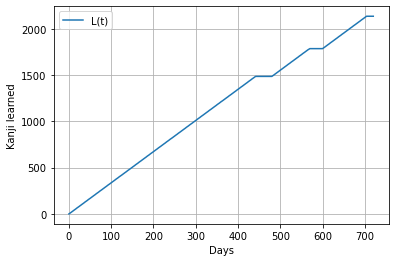
\includegraphics[scale=0.75]{2.png}
\caption{ภาพแสดงกราฟผลลัพธ์เชิงตัวเลขแบบทั่วไป}
\label{fig:graph1}
\end{figure}

\begin{figure}
\centering
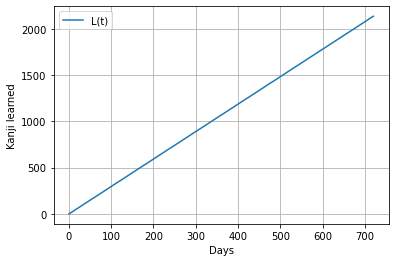
\includegraphics[scale=0.75]{3.png}
\caption{ภาพแสดงกราฟผลลัพธ์เชิงตัวเลขแบบพอดี}
\label{fig:graph2}
\end{figure}

\begin{figure}
\centering
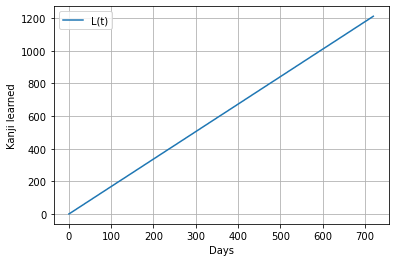
\includegraphics[scale=0.75]{4.png}
\caption{ภาพแสดงกราฟผลลัพธ์เชิงตัวเลขแบบไม่พอดี}
\label{fig:graph3}
\end{figure}

\begin{figure}
\centering
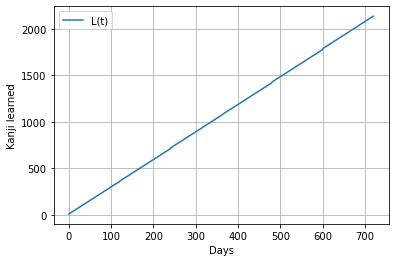
\includegraphics[scale=0.75]{5.png}
\caption{ภาพแสดงกราฟผลลัพธ์เชิงตัวเลขแบบพิเศษ}
\label{fig:graph4}
\end{figure}

\section{บทวิเคราะห์}
สำหรับแบบจำลองทางคณิตศาสตร์การเรียนรู้ตัวอักษรคันจิที่เราได้ทำมานั้น ยังคงเป็นเพียงแบบจำลองทางคณิตศาสตร์ที่อยู่ภายใต้เงื่อนไขหลักสูตรสาขาภาษาญี่ปุ่นของมหาวิทยาลัยธรรมศาสตร์เท่านั้น จึงทำให้มีคำถามที่น่าสนใจเกี่ยวกับตัวแบบจำลองทางคณิตศาสตร์ตัวนี้ว่า ถ้าเกิดเราจะแบ่งวิชาเรียนที่เกี่ยวข้องกับตัวอักษรคันจิในแบบอื่นๆ นอกเหนือจากหลักสูตรสาขาภาษาญี่ปุ่นของมหาวิทยาลัยธรรมศาสตร์ได้ไหม? โดยถ้ามองในมุมมองปัญหาจากข้อความข้างต้น เราจะพบว่าสิ่งที่ทำให้เกิดคำถามนี้ขึ้นมาเป็นเพราะว่าทุกๆ มหาลัยแต่ละมหาลัยก็มีหลักสูตรเป็นของตัวเอง บางมหาลัยอาจจะเปิดสอนวิชาที่เกี่ยวกับตัวอักษรคันจิเพียงแค่ 4 วิชา หรือ บางมหาลัยอาจจะเลือกสอนวิชาตัวอักษรคันจิโดยตรงก็มีให้เห็นได้ ดังนั้น การที่เราจะบรรลุเงื่อนไขแบบจำลองทางคณิตศาสตร์การเรียนรู้ตัวอักษรคันจิที่สามารถรองรับปัญหาในกรณีที่ต้องการทราบเวลาในการเรียนรู้ตัวอักษรคันจิเท่าไรจึงจะเรียนรู้ครบทุกตัวอักษรคันจิ และถ้าต้องเรียนรู้ตัวอักษรคันจิในเวลาที่จำกัดจะต้องเรียนรู้ตัวอักษรคันจิกี่ตัวต่อวันถึงจะเรียนรู้ตัวอักษรคันจิครบทุกตัว โดยที่มีวิชาเรียนเกี่ยวกับตัวอักษรคันจิแบบกำหนดเองได้ดังนี้ 
\begin{enumerate}
	\item พิจารณาสมการ $L_1(t)$ จนถึงสมการ $L_6(t)$ เราจะพบความสัมพันธ์ของตัวห้อย i กับตัวแปรต่างๆ และ การเพิ่มขึ้นของเวลาอย่างเป็นระบบ 
	\item มองสมการ $L_1(t)$ จนถึงสมการ $L_6(t)$ ให้อยู่ในรูป $L_i(t)$ เราจะได้สมการสำหรับทุกๆ $L_1(t)$ ถึง $L_6(t)$ ดังสมการด้านล่าง
\end{enumerate}
$$ L_n(t) = \sum_{i=1}^{n} \min \{J_i + K_i, \left\lfloor (1 - \beta)(K_{0,i} + \alpha{t - 120(i - 1)}) \right\rfloor\} \; ; t \in [120(n - 1),120n] $$ 
เพียงเท่านี้ เราจะได้สมการที่สามารถให้ใช้ทำแบบจำลองทางคณิตศาสตร์การเรียนรู้ตัวอักษรคันจิที่สามารถตอบโจทย์ปัญหาที่กล่าวมาได้ แต่ในส่วนของการตามหาจำนวนตัวอักษรคันจิที่ควรเรียนต่อวันภายใต้เงื่อนไขเวลาที่จำกัดในแบบจำลองทางคณิตศาสตร์นี้ก็มีแนวโน้มที่จะต้องใช้ข้อมูลจริงในการหาคำตอบร่วมด้วย

\section{สรุปผล}
จากการทำแบบจำลองทางคณิตศาสตร์การเรียนรู้ตัวอักษรคันจิ ทำให้เราพบว่าแบบจำลองทางคณิตศาสตร์ของเราสามารถบรรลุโจทย์การหาเวลาในการเรียนรู้ตัวอักษรคันจิเท่าไร จึงจะเรียนรู้ครบทุกตัวอักษรคันจิและการหาจำนวนตัวอักษรคันจิที่ควรเรียนต่อวันเมื่อมีเวลาในการเรียนที่จำกัด โดยที่ตัวแบบจำลองทางคณิตศาสตร์มีความสอดคล้องทางมิติ นอกจากนี้ แบบจำลองทางคณิตศาสตร์การเรียนรู้ตัวอักษรคันจิยังสามารถนำไปพิจารณาแนวโน้มในการเรียนรู้ตัวอักษรคันจิได้ด้วยว่าถ้าเราเรียนรู้ตัวอักษรคันจิประมาณเท่าใดจะทำให้เรียนตัวอักษรคันจิเร็วเกินไปหรือช้าเกินไปได้ แน่นอนว่าแบบจำลองทางคณิตศาสตร์การเรียนรู้ตัวอักษรคันจิของเราเองก็มีข้อกัดอยู่ เช่น ไม่สามารถบรรจุโจทย์กรณีการเรียนตัวอักษรคันจิมีผลต่อการจำตัวอักษรคันจิได้ กล่าวคือ แบบจำลองทางคณิตศาสตร์การเรียนรู้ตัวอักษรคันจิยังทำได้เพียงคาดคะเนผลลัพธ์ภายใต้เงื่อนไขการลืมตัวอักษรคันจิในปริมาณเท่าเดิมได้เท่านั้น ไม่สามารถคาดคะเนผลลัพธ์ภายใต้เงื่อนไขการลืมตัวอักษรคันจิในปริมาณที่เพิ่มมากขึ้นในแต่ละวันได้ เป็นต้น

\printbibliography

\end{document}